\chapter{Poincar\'e: Recurrence, Chance and the Crisis of Physics}
\label{ch:poincare}

\section{The other figure in Paris}

If Hilbert was the voice of the 1900 congress, Henri Poincar\'e was its presiding figure. He was president of the congress and spoke on the role of intuition and logic in mathematics; in the same week, at the International Congress of Physics held during the same Exposition, he addressed the relations between experimental and mathematical physics. He was forty six. He had already transformed celestial mechanics, created the qualitative theory of differential equations and algebraic topology, written the standard French treatises on thermodynamics, electromagnetism and probability, and examined, that spring, the thesis of Louis Bachelier.

Poincar\'e touched every part of the sixth problem. This chapter proves the theorems behind three of his contributions: recurrence, arbitrary functions and the Poincar\'e inequality.

\section{The three body problem and the prize}

In 1885 King Oscar II of Sweden and Norway announced a prize, organized by G\"osta Mittag Leffler, for the solution of one of four problems, the first being the representation of the motion of $n$ bodies under Newtonian gravitation by uniformly convergent series. Poincar\'e's memoir won in January 1889. While the memoir was being printed in \emph{Acta Mathematica}, Lars Edvard Phragm\'en raised a query that led Poincar\'e to discover a serious error: he had assumed that certain invariant curves, the stable and unstable manifolds of a periodic orbit, must coincide, and they need not. The printed copies were recalled at Poincar\'e's expense, which exceeded the value of the prize, and the corrected memoir appeared in 1890~\cite{poincare1890}. The correction contained the first glimpse of what is now called chaos: stable and unstable manifolds that intersect transversally, producing a homoclinic tangle of infinite complexity.

The memoir also contained the device that makes such phenomena visible, the surface of section. For a Hamiltonian system with two degrees of freedom the energy surface is three dimensional; recording the successive intersections of an orbit with a two dimensional transversal surface reduces the flow to an area preserving map of the plane. Figure~\ref{fig:hh} shows this map for the H\'enon Heiles Hamiltonian
\[
H = \tfrac12(p_x^2 + p_y^2) + \tfrac12(x^2+y^2) + x^2 y - \tfrac13 y^3
\]
at energy $E = 1/8$, a model introduced in 1964 to study whether galactic orbits possess a third integral~\cite{henonheiles1964}. Closed curves are invariant tori, remnants of integrability whose persistence under small perturbations is the subject of the theorem of Kolmogorov, Arnold and Moser~\cite{kolmogorov1954,arnold1963,moser1962}; the scattered dots are chaotic orbits that fill a region of apparently positive area. At this energy, three quarters of the escape energy, the perturbation is not small, and the picture is numerical evidence rather than a consequence of that theorem. Poincar\'e had foreseen the chaotic region in the homoclinic tangle of the memoir.

\begin{figure}[t]
\centering
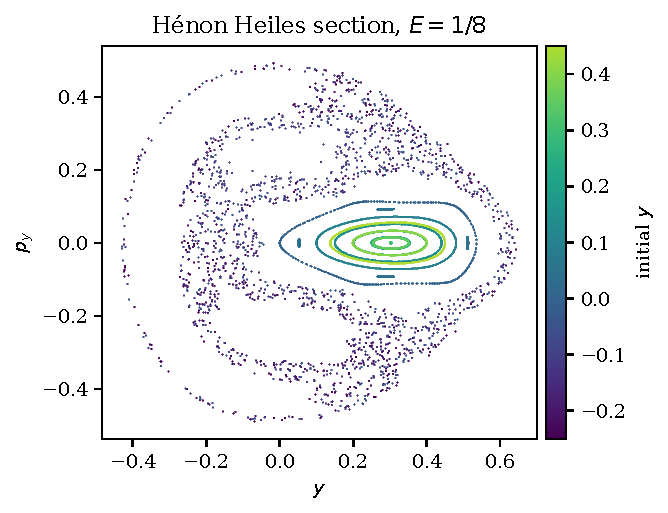
\includegraphics[width=0.78\textwidth]{henon_heiles}
\caption{Poincar\'e's surface of section for the H\'enon Heiles system at $E=1/8$, crossing $x=0$ with $p_x>0$. Fifteen orbits, started at $x=0$ and $p_y=0$ with $y$ equally spaced from $-0.25$ to $0.45$ and followed to time $2500$, are colored by initial $y$. Ten lie on invariant curves and five wander through a chaotic region.}
\label{fig:hh}
\end{figure}

\section{The recurrence theorem}

\begin{theorem}[Poincar\'e recurrence]
\label{thm:recurrence}
Let $(X,\mathcal{B},\mu)$ be a probability space and $T:X\to X$ a measurable map preserving $\mu$. For every $A\in\mathcal{B}$, almost every point of $A$ returns to $A$ infinitely often:
\[
\mu\big(\{x\in A: T^n x\in A \text{ for infinitely many } n\}\big) = \mu(A).
\]
\end{theorem}

\begin{proof}
Let $B = \{x\in A: T^n x\notin A \text{ for all } n\geq 1\}$. The sets $T^{-k}B$, $k\geq 0$, are pairwise disjoint: if $x\in T^{-j}B\cap T^{-k}B$ with $j<k$, then $y=T^j x\in B\subset A$ and $T^{k-j}y = T^k x\in B\subset A$, contradicting $y\in B$. Since $\mu(T^{-k}B) = \mu(B)$ and the total mass is one, $\sum_k \mu(B)\leq 1$ forces $\mu(B)=0$. A point $x\in A$ that returns to $A$ only finitely often has a last visit time $n\geq0$, where $n=0$ if it never returns, and then $T^n x\in B$. The set of such points is contained in $\bigcup_{n\geq0}T^{-n}B$, which is null.
\end{proof}

Poincar\'e proved the theorem for volume preserving flows in the memoir on the three body problem~\cite{poincare1890}, and Carath\'eodory gave a short proof for a general invariant measure~\cite{caratheodory1919}. For a Hamiltonian flow on a compact energy surface, Liouville's theorem supplies the invariant measure, and recurrence follows. Poincar\'e drew the consequence for kinetic theory in 1893~\cite{poincare1893}: a gas in a box, started from a state of low entropy, will return arbitrarily close to that state, and so the entropy cannot increase forever. In 1896 Ernst Zermelo, then Planck's assistant, turned this into a formal objection to Boltzmann's H theorem~\cite{zermelo1896}. Boltzmann's reply was that the recurrence times are so long as to be irrelevant. Kac made the reply quantitative~\cite{kac1947}.

\begin{theorem}[Kac's lemma]
\label{thm:kac_lemma}
Let $(X,\mathcal{B},\mu)$ be a probability space and $T:X\to X$ a measurable map preserving $\mu$ that is ergodic: every $B\in\mathcal{B}$ with $\mu(T^{-1}B\,\triangle\,B)=0$ has $\mu(B)\in\{0,1\}$ (Chapter~\ref{ch:ergodic} develops the notion). Let $A\in\mathcal{B}$ with $\mu(A)>0$ and let $\tau_A(x) = \inf\{n\geq 1: T^n x\in A\}$. Then
\[
\int_A \tau_A \dd\mu = 1,\qquad\text{equivalently}\qquad \E_\mu\big[\tau_A\mid A\big] = \frac{1}{\mu(A)},
\]
where $\E_\mu[\,\cdot\mid A]$ is the expectation under $\mu$ conditioned on $A$.
\end{theorem}

\begin{proof}
Let $S = \bigcup_{n\geq0}T^{-n}A$ be the set of points that enter $A$ at some time. Then $T^{-1}S\subset S$ and $\mu(T^{-1}S) = \mu(S)$, so $\mu(T^{-1}S\,\triangle\,S) = 0$. Since $S\supset A$ and $\mu(A)>0$, ergodicity gives $\mu(S) = 1$.

Let $\varphi(x) = \inf\{n\geq0:T^nx\in A\}$ be the entry time into $A$, so that $\{\varphi<\infty\} = S$ and $\{\varphi = 0\} = A$. Comparing the first visit to $A$ from $x$ with the first visit from $Tx$ gives $\tau_A(x) = 1+\varphi(Tx)$ for $x\in A$ and $\varphi(x) = 1+\varphi(Tx)$ for $x\notin A$. Put $E_k = \{\varphi = k\}$. The second relation says $E_{k+1} = T^{-1}E_k\setminus A$, and the first says $A\cap T^{-1}E_k = A\cap\{\tau_A = k+1\}$. Since $\mu(T^{-1}E_k) = \mu(E_k)$,
\[
\mu(E_{k+1}) = \mu(E_k) - \mu\big(A\cap\{\tau_A = k+1\}\big).
\]
As $\mu(E_0) = \mu(A) = \mu(A\cap\{\tau_A>0\})$, induction gives $\mu(E_k) = \mu(A\cap\{\tau_A>k\})$ for every $k\geq0$. Summing over $k$,
\[
1 = \mu(S) = \sum_{k\geq0}\mu(E_k) = \sum_{k\geq0}\mu\big(A\cap\{\tau_A>k\}\big) = \int_A\tau_A\dd\mu.
\]
The conditional form follows by dividing by $\mu(A)$. Ergodicity was used only to obtain $\mu(S) = 1$. Without it the computation gives $\int_A\tau_A\dd\mu = \mu(S)$, which for the identity map of a two point space with the uniform measure and $A$ one of the points is $\tfrac12$.
\end{proof}

For a mole of gas, the set of microstates in which, say, all molecules lie in the left half of the box has relative measure about $2^{-6\times 10^{23}}$. If the time one map $T$ of the gas is ergodic, Theorem~\ref{thm:kac_lemma} says that the expected return time to this set from a start in it is the reciprocal, $2^{6\times10^{23}}$ steps of $T$, a number with about $1.8\times10^{23}$ decimal digits, whereas the number of atoms in the observable universe, about $10^{80}$, has 81. Recurrence is a theorem; it is also irrelevant on every physical time scale. Chapter~\ref{ch:kinetic} treats an exactly solvable model, Kac's ring, in which the recurrence time is $2N$ and Boltzmann's law holds for times that are short compared with it (Figure~\ref{fig:kacring}). The ring map is a permutation of period $2N$ and is not ergodic, so Theorem~\ref{thm:kac_lemma} does not apply to it.

\section{The method of arbitrary functions}

How does chance arise in a deterministic world? Poincar\'e's answer, given in an essay of 1899~\cite{poincare1899} and in the second edition of the \emph{Calcul des probabilit\'es}~\cite{poincare1912calcul}, used a roulette wheel. The wheel is divided into many equal sectors, alternately red and black. The croupier gives it an initial velocity, and the final position is a deterministic but extremely sensitive function of that velocity. Poincar\'e argued that whatever the distribution of initial velocities, provided it is reasonably smooth, the probability of red will be close to one half. The probability is not in the dynamics and not in the croupier; it emerges from the interaction of a smooth density with a rapidly oscillating map. Borel gave the method a chapter of its own in a textbook of 1909~\cite{borel1909elements} and observed that continuity of the density suffices, Fr\'echet reduced the requirement to Riemann integrability in 1921~\cite{frechet1921}, Hopf recast it in the 1930s as a statement about the long time behavior of dynamical systems, related to mixing~\cite{hopf1934}, and Engel gave a comprehensive treatment~\cite{engel1992}. The following sharp version is elementary.

\begin{theorem}[Arbitrary functions]
\label{thm:arbitrary}
Let $X$ be a real random variable with density $g$ of total variation $V<\infty$. For $t>0$ and $a\in[0,1]$,
\[
\Big|\,\P\big(\{tX\}\in[0,a)\big) - a\,\Big|\leq \frac{a(1-a)\,V}{2t},
\]
where $\{\cdot\}$ denotes the fractional part. The bound is attained: for the uniform density on $[0,1]$, which has $V=2$, the error equals $a(1-a)/t$ whenever $t-a$ is a nonnegative integer.
\end{theorem}

\begin{proof}
For $a\in\{0,1\}$ both sides vanish, so let $0<a<1$. Partition $\R$ into the cells $I_n = [n/t,(n+1)/t)$ and split each into $I_n' = [n/t,(n+a)/t)$ and $I_n'' = [(n+a)/t,(n+1)/t)$, of lengths $a/t$ and $(1-a)/t$. Let $\bar g_n'$ and $\bar g_n''$ be the averages of $g$ over $I_n'$ and $I_n''$. Since $\{tX\}\in[0,a)$ exactly when $X\in I_n'$ for some $n$, and $\sum_n\int_{I_n}g = 1$,
\[
\begin{aligned}\P(\{tX\}\in[0,a)) - a &= \sum_{n\in\Z}\Big(\int_{I_n'}g - a\int_{I_n}g\Big)\\
&= \frac{a(1-a)}{t}\sum_{n\in\Z}\big(\bar g_n'-\bar g_n''\big),\end{aligned}
\]
where the last step uses $\int_{I_n'}g = \frac at\bar g_n'$ and $\int_{I_n}g = \frac at\bar g_n'+\frac{1-a}t\bar g_n''$. A density of bounded variation tends to zero at $\pm\infty$, so its Jordan decomposition is $g = g_+-g_-$ with $g_\pm$ nondecreasing and each of total increase $V/2$. For a nondecreasing function $h$ the average over $I_n'$ is at most $h((n+a)/t)$, the average over $I_n''$ is at least $h((n+a)/t)$, and both lie between the infimum and the supremum of $h$ over $I_n$. Hence $-\Delta_nh\leq\bar h_n'-\bar h_n''\leq0$, where $\Delta_nh$ is the increase of $h$ over $I_n$. Applied to $g_+$ and $g_-$ this gives $-\Delta_ng_+\leq\bar g_n'-\bar g_n''\leq\Delta_ng_-$, and since $\sum_n\Delta_ng_\pm\leq V/2$, the sum over $n$ has absolute value at most $V/2$.
\end{proof}

Theorem~\ref{thm:arbitrary} is an early and simple instance of a result that derives a probability law from a deterministic dynamics: the output law is insensitive to the input law, which may be regarded as a prior, because the dynamics stretches phase space. The rate $1/t$ can be improved for smoother densities. If $g$ is continuously differentiable and $g'$ has bounded variation $V'$, the Poisson summation formula gives $\P(\{tX\}\in[0,a)) - a = \sum_{k\neq0}\frac{e^{2\pi ika}-1}{2\pi ik}\,\hat g(kt)$, where $\hat g(\xi) = \int g(x)e^{-2\pi ix\xi}\dd x$, and two integrations by parts give $|\hat g(\xi)|\leq V'/(4\pi^2\xi^2)$. The error is then at most $\zeta(3)V'/(2\pi^3t^2)$. Poincar\'e insisted that every probability statement rests on a convention, a choice of prior; the method of arbitrary functions explains why, in physics, the choice often does not matter.

\section{Poincar\'e and inverse probability}

Poincar\'e was a Bayesian in the precise sense that he regarded the probability of causes as the fundamental problem of applied probability and held that it cannot be solved without a prior. In \emph{La science et l'hypoth\`ese} (1902) Poincar\'e calls the problems of the probability of causes the most important from the point of view of scientific applications and the essential problem of the experimental method~\cite{poincare1902}. The book states that the probability of a cause, given the observed effect, could not be calculated if a more or less justified convention did not supply in advance the probability of the cause, and that without such a convention the problem would have no meaning. The same reasoning applies to the inference of a physical law from observations: a curve drawn through measured points is the most probable law only because a regular law is judged more probable beforehand than an irregular one.

The most dramatic application was legal. In the Dreyfus affair the handwriting expert Alphonse Bertillon had argued, with a pseudo mathematical analysis of coincidences in the \emph{bordereau}, that Dreyfus was its author. Poincar\'e's letter, read at the Rennes court martial in 1899, criticized Bertillon's work for its lack of scientific foundation~\cite{mazliak2012}. In 1904 the Cour de cassation asked Darboux, Appell and Poincar\'e for a full report~\cite{darboux1904}. It opens with a short chapter on the probability of causes, which Mansuy and Mazliak describe as a small course on the correct use of the Bayes formula~\cite{mansuymazliak2005}. The report shows that Bertillon had computed the probability of four coincidences as $(0.2)^4$, which is the probability that four specified trials all produce a coincidence, whereas the probability of four coincidences among the twenty six trials available, which the report puts at about $0.7$, is some four hundred times larger, and that coincidences chosen because they were noticed prove nothing. It explains with two urns that the question is the probability of a cause given an observed effect, here forgery or natural writing, and that answering it requires the probability of the cause before the evidence. The authors held that in a question of this kind the prior is made of moral elements that escape calculation. They gave no probability of forgery and said only that the coincidences multiply the odds on forgery by some factor. The verdict against Dreyfus was annulled in 1906.

Poincar\'e also recorded the famous remark, which he attributed to Lippmann, that everyone believes in the normal law of errors: the experimenters because they think it is a theorem of mathematics, and the mathematicians because they think it is an experimental fact~\cite{poincare1912calcul}. The remark is a joke about foundations, and the sixth problem is the request to take the joke seriously. The central limit theorem, the maximum entropy characterization and the Maxwell characterization by rotation invariance and independence are three different mathematical reasons for the normal law, and each corresponds to a different physical hypothesis.

\section{Poincar\'e and Bachelier}

Poincar\'e's report on Bachelier's thesis~\cite{bachelier1900}, written in 1900, is short and appreciative~\cite{courtault2000}. He noted the originality of the approach, praised the derivation of the law of the price by a reasoning analogous to Fourier's theory of heat, and observed that the topic was somewhat removed from those usually treated by candidates. The thesis received the grade \emph{honorable}, which was respectable but not the highest~\cite{taqqu2001}. Bachelier's later career was difficult, and the work was largely neglected until Kolmogorov cited it in 1931~\cite{kolmogorov1931}. Samuelson, alerted by Savage, brought it to the attention of economists in the 1950s~\cite{taqqu2001}.

Bachelier showed that the probability density of a price with independent increments satisfies what he called the equation of radiation of probability, the heat equation. This is an early and influential appearance of the idea that a macroscopic diffusion is the law of a microscopic random motion, the idea Einstein made physical in 1905~\cite{einstein1905} and that Chapter~\ref{ch:brownian} develops.

\section{The quantum and the end of continuity}

In 1911 Poincar\'e attended the first Solvay conference in Brussels, devoted to radiation and the quanta. Returning to Paris he set himself a precise question: is the quantum hypothesis necessary to obtain Planck's law of black body radiation, or might a continuous mechanics with a suitable distribution of energies suffice? In a long paper of 1912~\cite{poincare1912quanta} he showed that it is necessary. The mathematical core is a uniqueness theorem for Laplace transforms. Let $\sigma$ be the measure on $[0,\infty)$ that describes how many states of a resonator of frequency $\nu$ have a given energy, so that at inverse temperature $\beta$ the partition function is $Z(\beta)=\int e^{-\beta E}\sigma(\dd E)$ and the mean energy is $-\frac{\dd}{\dd\beta}\log Z(\beta)$. Planck's law says that the mean energy is $h\nu/(e^{\beta h\nu}-1)$, where $h$ is Planck's constant. Integrating, $Z(\beta)=c\,(1-e^{-\beta h\nu})^{-1}=c\sum_{j\geq0}e^{-\beta jh\nu}$ for a constant $c$, and since a measure on $[0,\infty)$ is determined by its Laplace transform, $\sigma=c\sum_{j\geq0}\delta_{jh\nu}$: the energy of the resonator is concentrated on integer multiples of $h\nu$. A continuous distribution of energies, for which $\sigma$ has a density, cannot produce Planck's law, and the classical choice $\sigma(\dd E)\propto\dd E$ gives the mean energy $1/\beta$ and the Rayleigh Jeans law. Poincar\'e's own proof treats resonators exchanging energy with molecules at fixed total energy and is more delicate~\cite{prentis1995,mccormmach1967}, but it is a statement of the same kind about the support of a measure inferred from an observed law, and in that sense it is an inverse problem in exactly our sense. Ehrenfest reached a related conclusion in 1911~\cite{ehrenfest1911quanta}. Poincar\'e died in July 1912, a few months later. Chapter~\ref{ch:quantum} takes up the axiomatization of the quantum theory.

\section{The Poincar\'e inequality}

The rate at which a diffusion forgets its initial state is controlled by an inequality that bears Poincar\'e's name, after his 1890 paper on the partial differential equations of mathematical physics~\cite{poincare1890b}. The Gaussian case was proved by Nash~\cite{nash1958} and Chernoff~\cite{chernoff1981} with Hermite polynomials; the proof below uses the Ornstein Uhlenbeck semigroup instead.

\begin{theorem}[Gaussian Poincar\'e inequality]
\label{thm:gaussian_poincare}
Let $\gamma$ be the standard Gaussian measure on $\R^n$. For every $f\in L^2(\gamma)$ with weak gradient in $L^2(\gamma)$,
\[
\Var_\gamma(f)\leq \int |\nabla f|^2 \dd\gamma,
\]
with equality for linear $f$.
\end{theorem}

\begin{proof}
It suffices to prove the inequality for smooth $f$ such that $f$ and $\nabla f$ have polynomial growth: these functions are dense in the class of the statement for the norm $(\int f^2\dd\gamma+\int|\nabla f|^2\dd\gamma)^{1/2}$, and both sides of the inequality are continuous for that norm. Let $(P_t)$ be the Ornstein Uhlenbeck semigroup, $P_t f(x) = \E f(e^{-t}x + \sqrt{1-e^{-2t}}\,Z)$ with $Z\sim\gamma$. It is symmetric in $L^2(\gamma)$, has generator $\mathcal{L}f = \Delta f - x\cdot\nabla f$, satisfies $\int f\,\mathcal{L}f\dd\gamma = -\int|\nabla f|^2\dd\gamma$, and $P_t f\to\int f\dd\gamma$ in $L^2(\gamma)$. Differentiating under the integral sign gives the commutation $\nabla P_t f = e^{-t}P_t\nabla f$, and Jensen's inequality gives $|\nabla P_t f|^2\leq e^{-2t}P_t|\nabla f|^2$. Hence
\[
\begin{aligned}\Var_\gamma(f) &= -\int_0^\infty \frac{\dd}{\dd t}\int (P_t f)^2\dd\gamma\dd t\\
&= 2\int_0^\infty\!\!\int |\nabla P_t f|^2\dd\gamma\dd t\\
&\leq 2\int_0^\infty e^{-2t}\dd t\int |\nabla f|^2\dd\gamma,\end{aligned}
\]
using invariance $\int P_t g\dd\gamma = \int g\dd\gamma$. For $f(x) = a\cdot x$ both sides equal $|a|^2$.
\end{proof}

\begin{corollary}[Exponential convergence to equilibrium]
For the Ornstein Uhlenbeck semigroup, $\|P_t f - \int f\dd\gamma\|_{L^2(\gamma)}\leq e^{-t}\|f - \int f\dd\gamma\|_{L^2(\gamma)}$.
\end{corollary}

\begin{proof}
Write $h(t) = \Var_\gamma(P_t f)$. Then $h'(t) = -2\int |\nabla P_t f|^2\dd\gamma\leq -2h(t)$ by the theorem applied to $P_t f$, and Gr\"onwall's lemma gives $h(t)\leq e^{-2t}h(0)$.
\end{proof}

The best constant $C$ in a Poincar\'e inequality $\Var_\pi(f)\leq C\,\mathcal{E}(f,f)$, where $\mathcal{E}(f,f) = -\int f\,\mathcal{L}f\dd\pi$ is the Dirichlet form of the generator, is the reciprocal of the spectral gap $\lambda_1$ of $-\mathcal{L}$; for the Ornstein Uhlenbeck process both equal one. Poincar\'e inequalities and their logarithmic strengthening, the log Sobolev inequality of Theorem~\ref{thm:lsi}, give the rates of convergence to equilibrium for the Ornstein Uhlenbeck flow in Chapter~\ref{ch:entropy} and for Kac's model in Chapter~\ref{ch:kinetic}. The same constant governs the efficiency of Markov chain Monte Carlo: for a reversible chain the asymptotic variance of an ergodic average is at most $(2/\lambda_1-1)\Var_\pi(f)$, where $\lambda_1$ is the spectral gap of the chain (Chapter~\ref{ch:ergodic}), so a Poincar\'e constant is a statement about how much computation inference costs.

\section{The conjecture and Perelman's entropy}

In the fifth supplement to \emph{Analysis Situs}, published in 1904~\cite{poincare1904}, Poincar\'e asked whether a closed three dimensional manifold with trivial fundamental group must be homeomorphic to the three sphere. The question became the most famous problem in topology. Hamilton proposed in 1982 to attack it with the Ricci flow $\partial_t g = -2\Ric(g)$, a nonlinear heat equation for the metric~\cite{hamilton1982}. Perelman completed the program in three preprints of 2002 and 2003~\cite{perelman2002,perelman2003a,perelman2003b}, and the first of them introduced a functional that Perelman called an entropy. Let $(M,g)$ be a closed $n$ dimensional Riemannian manifold with scalar curvature $R$ and Riemannian volume element $\dd\,\mathrm{vol}$, let $f$ be a smooth function on $M$ and let $\tau>0$, with $f$ normalized by $\int_M(4\pi\tau)^{-n/2}e^{-f}\dd\,\mathrm{vol} = 1$. Perelman's functional is
\[
\mathcal{W}(g,f,\tau) = \int_M \big[\tau\big(R + |\nabla f|^2\big) + f - n\big]\,(4\pi\tau)^{-n/2}e^{-f}\dd\,\mathrm{vol}.
\]
Perelman remarked on the analogy with Boltzmann's entropy and with the thermodynamics of the heat kernel. In Chapter~\ref{ch:entropy} we show that on flat space $\mathcal{W}$ is exactly the combination of Shannon entropy and Fisher information that appears in de Bruijn's identity, that its monotonicity along the heat flow is a probabilistic statement about Gaussian convolution, and that its nonnegativity is the log Sobolev inequality (Theorem~\ref{thm:perelman_flat}). On a curved manifold $\mathcal{W}$ also contains the scalar curvature, which is why the identification with Shannon entropy and Fisher information holds only on flat space. Perelman's proof of the conjecture uses the monotonicity of $\mathcal{W}$ to show that the Ricci flow does not collapse locally, and then needs surgery at singular times~\cite{perelman2003a} and the finite extinction time of the flow~\cite{perelman2003b}; Kleiner and Lott give a detailed exposition of the first two preprints~\cite{kleinerlott2008}.

\section{Poincar\'e's shuffles: random walks on groups}

The second edition of \emph{Calcul des probabilit\'es}~\cite{poincare1912calcul} contains, in a chapter of miscellaneous questions added in 1912, a discussion of card shuffling that anticipates the modern theory of random walks on groups. Poincar\'e asked why repeated shuffles produce a deck in which every order is equally likely, and he answered by an argument from the theory of groups that refers to the work of Frobenius and Cartan; Mazliak~\cite{mazliak2012} describes it. The modern form is the following theorem.

\begin{theorem}[Convergence of random walks on finite groups]
\label{thm:random_walk_groups}
Let $G$ be a finite group and $Q$ a probability measure on $G$. The convolution powers $Q^{*n}$ converge to the uniform distribution $U$ on $G$ if and only if the support of $Q$ generates $G$ and is not contained in a coset of a proper normal subgroup. In that case, for every irreducible unitary representation $\rho\neq1$ the Fourier transform $\hat Q(\rho) = \sum_gQ(g)\rho(g)$ has spectral radius strictly less than one. Moreover, with $\|\mu-\nu\|_{TV} = \max_A|\mu(A)-\nu(A)|$,
\[
\|Q^{*n}-U\|_{TV}^2\leq\frac14\sum_{\rho\neq1}d_\rho\,\tr\big(\hat Q(\rho)^n(\hat Q(\rho)^n)^*\big),
\]
where the sum runs over the nontrivial irreducible unitary representations of $G$ up to equivalence and $d_\rho$ is the dimension of $\rho$.
\end{theorem}

\begin{proof}
If the support of $Q$ lies in a proper subgroup $H$, or in a coset $aN$ of a proper normal subgroup $N$, then $Q^{*n}$ gives mass one to $H$, or to the coset $a^nN$, which has $U$ mass at most $\frac12$. Then $\|Q^{*n}-U\|_{TV}\geq\frac12$ for every $n$, and there is no convergence. Now assume that the support generates $G$ and lies in no coset of a proper normal subgroup, and let $\rho\neq1$ be irreducible and unitary. Then $\hat Q(\rho)$ is a contraction. Suppose $\hat Q(\rho)v = \lambda v$ with $|\lambda| = 1$ and $|v| = 1$. Since $\lambda v$ is an average of the unit vectors $\rho(g)v$ for $g$ in the support, and the unit ball of a Hilbert space is strictly convex, $\rho(g)v = \lambda v$ for every $g$ in the support. Every element of the finite group $G$ is a product of elements of the support, so $v$ is an eigenvector of every $\rho(g)$. Irreducibility forces $\dim\rho = 1$, so $\rho$ is a nontrivial character $\chi$ with $\chi(g) = \lambda$ on the support, which then lies in a coset of the proper normal subgroup $\ker\chi$, contrary to assumption. Hence $\hat Q(\rho)$ has spectral radius less than one and $\hat Q(\rho)^n\to0$. The Fourier transform turns convolution into multiplication, $\widehat{Q^{*n}}(\rho) = \hat Q(\rho)^n$, and $\hat U(\rho) = 0$ for $\rho\neq1$. The displayed bound is the upper bound lemma of Diaconis and Shahshahani~\cite{diaconisshahshahani1981,diaconis1988}: Cauchy Schwarz turns total variation into an $L^2$ distance, and the Plancherel theorem for $G$ expresses the latter in terms of Fourier coefficients. Its right side is a finite sum of terms that tend to zero.
\end{proof}

The spectral radius cannot be replaced by the operator norm. On $S_3$ the measure uniform on $\{(12),(123)\}$ satisfies the conditions of the theorem, so it converges to uniform, but $\hat Q(\rho)$ has operator norm one on the two dimensional representation, with spectral radius $\frac12$. Poincar\'e did not compute rates, but the structure of his argument, a spectral gap on each nontrivial representation, is in our reading that of the theorem. Diaconis and Shahshahani showed in 1981 that random transpositions mix a deck of $n$ cards after about $\frac12n\log n$ steps~\cite{diaconisshahshahani1981}, and Bayer and Diaconis showed in 1992 that seven riffle shuffles suffice for a deck of fifty two~\cite{bayerdiaconis1992}. The method of arbitrary functions explains how a physical process forgets its initial condition; the random walk theorem explains how a sequence of independent randomizations forgets it. Both are theorems about convergence to a uniform law, and both are ancestors of the Markov chain Monte Carlo methods of Chapter~\ref{ch:spins}.

\section{The Maxwell, Poincar\'e and Borel lemma}

\begin{theorem}[Maxwell, Poincar\'e and Borel]
\label{thm:sphere_lemma}
Let $X^{(n)}$ be uniformly distributed on the sphere $\{x\in\R^n:|x|^2 = n\}$. For each fixed $k$ the law of the first $k$ coordinates $(X^{(n)}_1,\dots,X^{(n)}_k)$ converges in total variation to the standard Gaussian law on $\R^k$.
\end{theorem}

\begin{proof}
Let $Z$ be standard Gaussian in $\R^n$. By rotation invariance, $X^{(n)}\eqd\sqrt n\,Z/|Z|$. The first $k$ coordinates equal $Z_{1:k}\cdot\sqrt{n}/|Z|$, and $|Z|^2/n\to1$ almost surely by the law of large numbers. This gives convergence in law. For total variation, let $n>k$. The first $k$ coordinates have the density
\[
\begin{aligned}f_n(x) &= c_{n,k}\Big(1-\frac{|x|^2}{n}\Big)^{(n-k-2)/2},\quad |x|^2<n,\\
c_{n,k} &= \frac{\Gamma(n/2)}{(\pi n)^{k/2}\,\Gamma((n-k)/2)},\end{aligned}
\]
obtained by integrating over the sphere of radius $\sqrt{n-|x|^2}$ in $\R^{n-k}$, where $c_{n,k}$ is the constant that makes $f_n$ a probability density. By Stirling's formula $\Gamma(n/2)/\Gamma((n-k)/2)\sim(n/2)^{k/2}$, so $c_{n,k}\to(2\pi)^{-k/2}$, and $(1-|x|^2/n)^{(n-k-2)/2}\to e^{-|x|^2/2}$. Hence $f_n$ converges pointwise to the standard Gaussian density on $\R^k$. Since all these functions are probability densities, Scheff\'e's lemma upgrades pointwise convergence to convergence in total variation.
\end{proof}

The lemma is the microcanonical derivation of the Maxwellian: a gas with fixed total kinetic energy, uniformly distributed over the energy sphere, has Gaussian one particle velocities in the limit. It also underlies Kac's model in Chapter~\ref{ch:kinetic}, whose state space is exactly this sphere, and it is a relative of the concentration of measure phenomenon that L\'evy studied and that Milman later made a pillar of high dimensional geometry. The result is usually attributed to Poincar\'e, but Diaconis and Freedman could not find it in Poincar\'e's work~\cite{diaconisfreedman1987}. The earliest probabilistic statement they located is in Borel~\cite{borel1914}, who had studied the uniform measure on a ball of velocities in 1906~\cite{borel1906}, and they point to Maxwell for the idea. Their quantitative version gives a total variation bound of order $k/n$, the rate of the finite de Finetti theorem of Chapter~\ref{ch:axioms} for finitely many values.

\section{Poincar\'e on kinetic theory}

The paper of 1906, \emph{R\'eflexions sur la th\'eorie cin\'etique des gaz}~\cite{poincare1906}, examines the argument of Gibbs for the second law~\cite{gibbs1902} and distinguishes two hypotheses about probability. In the discontinuous hypothesis one has a very large number of similar systems, such as the molecules of a one dimensional gas, whose initial states are known exactly, and the probability of a region of phase space is the fraction of the systems that lie in it. In the continuous hypothesis the initial state of a single system is known only through a probability density. Under the first hypothesis the entropy integral is infinite, and the paper adopts the second. It also distinguishes the fine entropy, the limit of the cell entropies as the cells shrink, from the coarse entropy computed with cells so small that ordinary methods of observation cannot tell two states within a cell apart. It proves that the fine entropy is constant in time, so that any increase must come from coarse graining, and that, in the sign convention in which entropy increases, the coarse entropy is never smaller than the fine entropy. Gibbs had made the same point in the \emph{Elementary Principles}~\cite[Chapter~XII]{gibbs1902} with the picture of a coloring matter stirred through an incompressible liquid: its density measured on cells of fixed size tends to a uniform limit, although the density carried along with the liquid never changes.

These remarks are consistent with the structure of Lanford's theorem (Theorem~\ref{thm:lanford})~\cite{lanford1975}. The Boltzmann entropy that increases is the entropy of the one particle marginal, a coarse grained quantity; the Gibbs entropy of the full $N$ particle law is conserved; and the difference between them measures correlations created by collisions, which are invisible in the limit because they concentrate on a set of vanishing measure. In the language of Chapter~\ref{ch:axioms}, chaos is lost at finite $N$ and recovered in the limit, and Poincar\'e's two hypotheses correspond to the empirical measure of one gas and the de Finetti measure over gases.

\section{Poincar\'e and the theory of errors}

Poincar\'e's \emph{Calcul des probabilit\'es}~\cite{poincare1912calcul} also contains a careful discussion of Gauss's derivation of the normal law of errors. Gauss had shown in 1809~\cite{gauss1809} that if the arithmetic mean is always the most probable value of a location parameter, then the error law must be Gaussian. Poincar\'e examined the argument, noted that it presupposes a uniform prior on the location, and gave a version in which the prior is explicit and, with enough observations, does not affect the conclusion; Mazliak~\cite{mazliak2012} describes this analysis. It is an early instance of the observation that characterizations of the normal law by the optimality of the sample mean are statements about Bayes estimators under flat priors. In modern terms, the Gaussian is the only location family for which the sample mean is the maximum likelihood estimate of the location for every sample size, and under a flat prior the maximum likelihood estimate is the posterior mode. Teicher gave a rigorous proof that needs only continuity of the density and the property for samples of sizes two and three~\cite{teicher1961}. The three reasons for the normal law listed earlier in this chapter are thereby joined by a fourth, Gauss's: the Gaussian is the error law that makes averaging optimal.

\section{Poincar\'e and Hilbert}

Hilbert and Poincar\'e represented different philosophies of foundations. Hilbert's axiomatic method sought consistent formal systems from which theories could be deduced. Poincar\'e's conventionalism held that the axioms of geometry and mechanics are neither synthetic truths nor experimental facts but conventions, chosen for convenience and guided by experience; and he distrusted the formal turn in logic, which he satirized in his debates with Russell and Couturat. Yet on the sixth problem their views converge more than they diverge. Hilbert asked for the limiting process from atoms to continua. Poincar\'e had shown that the approach to equilibrium cannot hold for every initial condition, because of recurrence and reversibility, and that statements of this kind can hold for every smooth probability law on the initial conditions, as the method of arbitrary functions shows. The paper of 1906 makes the point for a very large number of small planets on circular orbits: the longitudes become uniformly distributed for every smooth law of the initial data, the recurrence time grows with the number of planets and is infinite in the limit, and an initial distribution that is not smooth, such as planets placed on a line, leaves a latent organization, a spiral wound too tightly to be seen, which a coarse observer takes for uniformity~\cite{poincare1906}. Boltzmann answered the objections of Loschmidt and Zermelo by moving from individual trajectories to probabilities. The modern answer to Hilbert, a limit theorem for the empirical measure under a probability law on initial conditions, as the number of particles grows and the time is held fixed, is due to Kac~\cite{kac1956} and, for hard spheres, Lanford~\cite{lanford1975} (Chapter~\ref{ch:kinetic}); it joins Hilbert's limit with Poincar\'e's probability measures.

The Bayesian reading adds one more convention to Poincar\'e's list: the prior on initial conditions. Poincar\'e had written that the probability of causes requires a hypothesis about prior probabilities; we add that the hypothesis can be checked, refined and computed with, and that the method of arbitrary functions explains when it washes out.

\section*{Exercises}
\begin{enumerate}
\item For the circle rotation $x\mapsto x+\alpha$ modulo one with $\alpha$ irrational, verify recurrence directly and compute the expected return time to an interval of length $\delta$ started uniformly in it.
\item Let $X$ be exponential with rate $\lambda$. Compute $\P(\{tX\}<\frac12)$ exactly and compare the error with the bound of Theorem~\ref{thm:arbitrary}.
\item Show that the Gaussian Poincar\'e inequality is an equality for the Hermite polynomial of degree one, and compute the ratio $\int|f'|^2\dd\gamma/\Var_\gamma(f)$ for the Hermite polynomial $\mathrm{He}_k$ of degree $k$ on $\R$.
\item Let $Q$ on $S_3$ give weight $\frac13$ to the identity and $\frac29$ to each of the three transpositions. Compute $\hat Q(\rho)$ for the two dimensional irreducible representation and for the sign representation, and find the rate of convergence to uniform. Explain why the walk that picks one of the three transpositions uniformly does not converge.
\item Derive the density of the first $k$ coordinates of a uniform point on the sphere of radius $\sqrt n$ in $\R^n$.
\end{enumerate}


\section*{Notes}

Barrow Green~\cite{barrowgreen1997} tells the story of the King Oscar prize and the error in detail. Gray~\cite{gray2013} is a scientific biography of Poincar\'e. The Darboux, Appell and Poincar\'e report on Bertillon~\cite{darboux1904} is introduced by Mansuy and Mazliak~\cite{mansuymazliak2005}; Taroni, Champod and Margot~\cite{taroni1998} survey the early history of Bayesian reasoning in forensic science. We have paraphrased the report's argument. Poincar\'e's quantum paper is analyzed by McCormmach~\cite{mccormmach1967} and Prentis~\cite{prentis1995}. Mazliak~\cite{mazliak2012} surveys Poincar\'e's work on probability. For the method of arbitrary functions see von Plato~\cite{vonplato1994} and Engel~\cite{engel1992}; Diaconis, Holmes and Montgomery~\cite{diaconis2007coin} apply the same reasoning to coin tossing and find a small but real bias toward the side facing up.
